\documentclass[a4paper,11pt]{article}
\pagestyle{plain}
\usepackage[T1,T2A]{fontenc}
\usepackage[utf8]{inputenc}
\usepackage[english,russian]{babel}
\usepackage{amssymb}
\usepackage{verbatim}
\usepackage{subfig}
\usepackage{hyperref}
\usepackage{graphicx}
\DeclareGraphicsExtensions{.png}
\author{Dmitriy Sukharev}
\title{Краткое описание системы Apache Hadoop}
\date{October 13, 2012}
\begin{document}
\section{Краткое описание системы Apache Hadoop}
Apache Hadoop -- набор программных средств для разработки и выполнения распределённых программ, работающих на кластерах
из сотен и тысяч узлов. Используется для реализации поисковых и контекстных механизмов многих высоконагруженных
веб-сайтов, в том числе, для Yahoo!, Facebook и Last.fm\cite{fb}\cite{powered-by}.

Основан на двух статьях, изданных корпорацией Google Inc.:
\begin{enumerate}
    \item The Google File System\cite{gfs} -- в статье описывается проприетарная распределенная файловая система GFS,
          предназначенная для работы распределенных приложений, обрабатывающих большое количество данных (порядка сотен
          терабайт).
    \item MapReduce: Simplified Data Processing on Large Clusters\cite{mapreduce} -- в статье описывается модель
          распределённых  вычислений, используемая для параллельных вычислений над очень большими, несколько петабайт,
          наборами данных в компьютерных кластерах.
\end{enumerate}

Основываясь на этих двух идеях Apache Hadoop состоит из 3 подпроектов:
\begin{enumerate}
    \item Hadoop HDFS -- файловая система, предназначенная для хранения файлов больших размеров, поблочно распределённых
          между узлами вычислительного кластера. Open-source аналог GFS.
    \item Hadoop MapReduce -- реализация описанного в \cite{mapreduce} проприетарного решения. Корпорация Google
          предоставила Apache Software Foundation права на использование технологии MapReduce.
    \item Hadoop Common -- сюда входят библиотеки управления файловыми системами, поддерживаемыми Hadoop и сценарии
          создания необходимой инфраструктуры и управления распределённой обработкой.
\end{enumerate}

\subsection{Hadoop HDFS (Википедия)}
HDFS (Hadoop Distributed File System) -- файловая система, предназначенная для хранения файлов больших размеров,
поблочно распределённых между узлами вычислительного кластера. Все блоки в HDFS (кроме последнего блока файла) имеют
одинаковый размер, и каждый блок может быть размещён на нескольких узлах, размер блока и коэффициент репликации
(количество узлов, на которых должен быть размещён каждый блок) определяются в настройках на уровне файла. Благодаря
репликации обеспечивается устойчивость распределённой системы к отказам отдельных узлов. Файлы в HDFS могут быть
записаны лишь однажды (модификация не поддерживается), а запись в файл в одно время может вести только один процесс.
Организация файлов в пространстве имён -- традиционная иерархическая: есть корневой каталог, поддерживается вложение
каталогов, в одном каталоге могут располагаться и файлы, и другие каталоги.

Развёртывание экземпляра HDFS предусматривает наличие центрального узла имён (англ. name node), хранящего метаданные
файловой системы и метаинформацию о распределении блоков, и серии узлов данных (англ. data node), непосредственно
хранящих блоки файлов. Узел имён отвечает за обработку операций уровня файлов и каталогов — открытие и закрытие файлов,
манипуляция с каталогами, узлы данных непосредственно отрабатывают операции по записи и чтению данных. Узел имён и узлы
данных снабжаются веб-серверами, отображающими текущий статус узлов и позволяющими просматривать содержимое файловой
системы. Административные функции доступны из интерфейса командной строки.

\subsection{Hadoop MapReduce}
Разработчику приложения для Hadoop MapReduce необходимо реализовать два интерфейса:
\begin{enumerate}
    \item Mapper -- принимает на вход пару <ключ, значение>, выполняя над ней преобразования, возвращает множество пар
          <ключ, значение>. Типы входящих и исходящих ключей, и входящих и исходящих значений могут не совпадать.
          Например в задаче подсчета количества слов во множестве документов, на вход Mapper'a подается пара
          <идентификатор документа, текст документа>, на выходе -- возвращается множество пар <слово, счетчик этого
          слова в документе>. Каждый Mapper выполняется в отдельном потоке, в отдельной Java Virtual Machine. Mapper'ы
          распределяются по узлам кластера равномерно. На узле может выполняться один или более mapper'ов. Стандартными
          подходами разбиения исходных данных по узлам является либо разбиение по документам (если данные содержатся во
          множестве файлов), либо разбиение по строчкам (если данные содержатся в одном файле).
    \item Reducer -- принимает на вход пару <ключ, список значений>, выполняя над ней преобразования, возвращает одно
          или больше значений, соответсвующих заданному ключу. Типы входящих и исходящих значений могут не совпадать.
          Например в задаче подсчета количества слов во множестве документов, на вход Reducer'a подается пара
          <cлово, список счетчиков этого слова в документах, которые обрабатывали разные Mapper'ы>, на выходе --
          возвращается единственное число -- сколько раз заданное слово встречается во всех документах. Каждый Mapper
          выполняется в отдельном потоке, в отдельной Java Virtual Machine. Reducer'ы распределяются по узлам кластера
          равномерно. На узле может выполняться один или более reducer'а. В приведенном примере количество reducer'ов
          равняется количеству уникальных слов во всех документах исходной выборки.
\end{enumerate}

Данный механизм позволяет свести к минимуму количество необходимых синхронизаций. На Рис.~\ref{fig:mapreduce} показана
схема выполнения задачи с применением механизма MapReduce. Следует отметить синхронизация узлов происходит всего один
раз -- во время этапа shuffle, в процессе которого пары, являющиеся результатом работы Mapper'ов, равномерно
распределяются по вычислительным узлам. При этом также происходит группирование множества пар <ключ, значение> с
одинаковым ключем в единственную пару <ключ, список значений>.

\begin{figure}[h!]
  \centering
  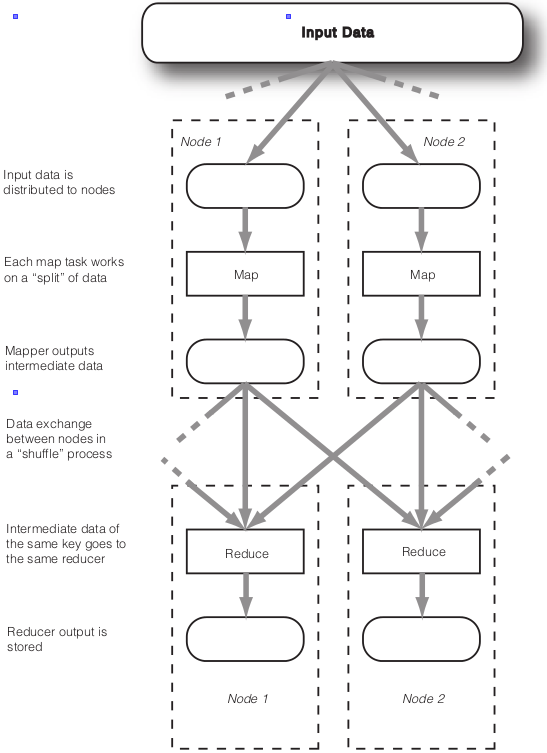
\includegraphics[height=350px]{res/mapreduce.png}
  \caption{Иллюстрация работы механизма MapReduce}
  \label{fig:mapreduce}
\end{figure}

Написание приложений под Apache Hadoop существенно отличается от написания приложений под другие системы. Связано это
с тем, что алгоритм нужно адаптировать под механизм MapReduce. Если задача с подсчетом количества слов в файлах хорошо
адаптируется под этот механизм, то, например, задачи, которые в результе возвращают единственное значение для
единтсвенного ключа могут вызвать у начинающего разработчика замешательство. Например мне было непонятно как можно
вычислить сумму квадратов большого количества чисел, пришлось спрашивать\cite{sum_of_squares}.

Всю свою эффективность механизм MapReduce начинает показывать при обработке данных начиная от сотен гигабайт
\cite[p.~6]{oreilly}.

\subsection{Архитектурные компоненты Apache Hadoop}
Hadoop кластер состоит из следующих архитектурных компонент (демонов):
\begin{enumerate}
  \item NameNode
  \item DataNode
  \item Secondary NameNode
  \item JobTracker
  \item TaskTracker
\end{enumerate}

Первые три в большей степени относятся к механизму хранения данных (HDFS), последние два -- к механизму организации
вычислений (MapReduce). На Рис~\ref{fig:daemons_2layers} показано распределение Hadoop демонов на вычислительные и
хранения данных.

Кроме того, демоны делятся на управляющие (master), и исполняющие (slave).

Рассмотрим каждую из компонент.

\begin{figure}[h!]
  \centering
  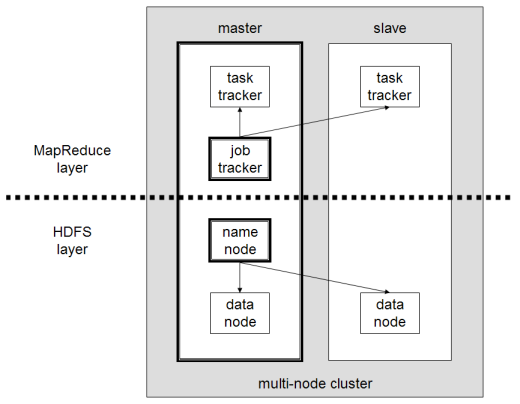
\includegraphics[height=200px]{res/daemons_2layers.png}
  \caption{Распределение Hadoop демонов на вычислительные и хранения данных}
  \label{fig:daemons_2layers}
\end{figure}


\subsubsection{NameNode}
Это наиболее важный из демонов Hadoop кластера. Является управляющим по отношению к исполняющим DataNode демонам.
Выполняет управление файловой системой HDFS. В частности, поскольку файлы разбиваются на блоки по 64 МБ, ведет учет
того как файлы разбиты на блоки, какие блоки находятся на каких узлах, и отслеживает "здоровье" файловой системы
в целом.

Поскольку функцией NameNode является управление памятью и операциями ввода вывода, то чтобы снизить нагрузку на этот
узел, он зачастую не хранит пользовательские данные и не выполняет вычислительные задачи.

Во всем кластере запущен всего один демон NameNode. Таким образом неприятным моментом является высокая важность
этой компоненты системы, поскольку она является единственной компонентой, отказ которой приводит к отказу всего
Hadoop кластера. При отказе любой другой компоненты функционирование системы сохраняется. В Facebook для избежания
отказа всего кластера при отказе NameNode используют модифицированную версию Apache Hadoop\cite{fb}.

\subsubsection{DataNode}
На каждом исполняющем (slave) узле системы выполняется демон DataNode. Он позволяет "рядовому" узлу работать с
распределенной файловой системой, быть её составной частью. При этом происходит обычное чтение или запись HDFS блоков
в файлы локальной файловой системы узла. При чтении или записи файла в HDFS, файл разбивается на блоки, и NameNode
определяет какому узлу соответствует какой блок.

На Рис.~\ref{fig:namenode_datanode} показан пример размещения двух файлов в HDFS. Первый занимает 3 блока, второй --
2 блока. При этом в настройках HDFS выставлена тройная репликация данных, поэтому каждый блок повторяется 3 раза.

Между DataNode и NameNode узлом выполняется heartbeat.

\begin{figure}[h!]
  \centering
  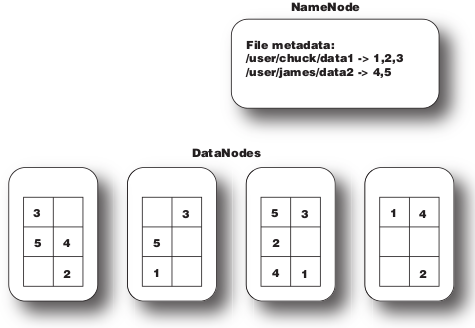
\includegraphics[height=200px]{res/namenode_datanode.png}
  \caption{Пример размещения файлов в HDFS}
  \label{fig:namenode_datanode}
\end{figure}

\subsubsection{Secondary NameNode}
Хранит снэпшоты информации о файловой системе с NameNode. В отличии от последней не отслеживает изменения ФС в реальном
времени, вместо этого всего лишь выполняет снимки с NameNode с заданной в конфигурации периодичностью. Во всем кластере
запущен всего один демон Secondary NameNode.

Secondary NameNode позволяет уменьшить время простоя системы и потери информации в случае отказа NameNode. Однако в
случае отказа NameNode необходимо вручную переконфигурировать кластер для использования Secondary NameNode как
первичного NameNode.

\subsubsection{JobTracker}
Является промежуточным звеном между пользовательским приложением и Hadoop. Как только пользователь сабмитит задачу
на кластер, JobTracker определяет какие файлы необходимо обрабатывать, назначает разные задачи на узлы и отслеживает
выполнение всех задач. Если какая-либо задача "упала", JobTracker автоматически перезапустит эту задачу, возможно, на
другом узле (в рамках заданного максимального количества перезапусков). Во всем кластере запущен всего один демон
JobTracker. Является управляющим по отношению к исполняющим TaskTracker демонам.

\subsubsection{TaskTracker}
Выполняется на каждом исполняющем (slave) узле системы. В то время как JobTracker отслеживает выполнение всей задачи
целиком, TaskTracker"ы управляют выполнением и выполняют отдельные задачи на исполняющих (slave) узлах
(Рис.~\ref{fig:jobtracker_tasktracker}).

\begin{figure}[h!]
  \centering
  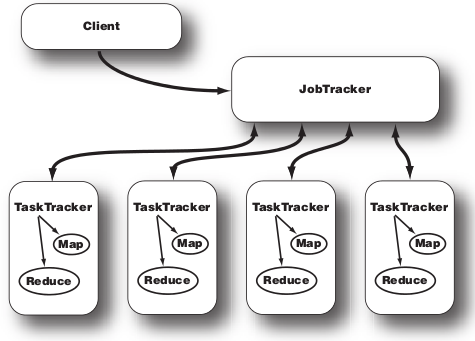
\includegraphics[height=200px]{res/jobtracker_tasktracker.png}
  \caption{Взаимодействие между JobTracker и TaskTracker демонами}
  \label{fig:jobtracker_tasktracker}
\end{figure}

TaskTracker должен постоянно взаимодействовать с JobTracker'ом. Если JobTracker не получает heartbeat от TaskTracker'a
в заданный интервал времени, он считает TaskTracker "упавшим" и переназначит соответствующую задачу на другой узел
кластера.

\subsubsection{Топология Hadoop кластера}
Зачастую Hadoop кластер имеет топологию представленную на Рис.~\ref{fig:master_slaves_cluster}. Однако в зависимости
от загруженности кластера демоны разносят по узлам, или, наоборот, запускают на меньшем количестве узлов. Так NameNode
и JobTracker при высокой загруженности кластера рекомендуют разносить по разным узлам. При малой же загруженности 
Secondary NameNode иногда размещают на исполнительном (slave) узле. Кроме того для разрабки приложений под Hadoop
существует возможность запускать все демоны на одном узле.

\begin{figure}[h!]
  \centering
  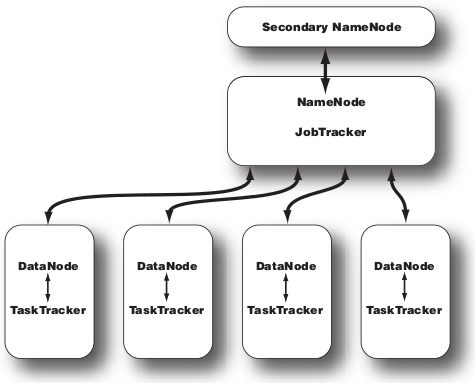
\includegraphics[height=200px]{res/master_slaves_cluster.png}
  \caption{Типичная топология Hadoop кластера}
  \label{fig:master_slaves_cluster}
\end{figure}

\section*{Полезные ссылки}
\begin{enumerate}
  \item \href{http://hadoop.apache.org/docs/stable/}{Сайт документации Apache Hadoop}
  \item \href{http://ru.wikipedia.org/wiki/Hadoop}{Статья википедии об Apache Hadoop}
\end{enumerate}

\begin{thebibliography}{4}
    \bibitem{fb}
        \href{http://www.facebook.com/notes/facebook-engineering/looking-at-the-code-behind-our-three-uses-of-apache-hadoop/468211193919}{http://www.facebook.com/notes/facebook-engineering/looking-at-the-code-behind-our-three-uses-of-apache-hadoop/468211193919}
    \bibitem{powered-by}
        \href{http://wiki.apache.org/hadoop/PoweredBy}{http://wiki.apache.org/hadoop/PoweredBy}
    \bibitem{gfs}
        \href{http://research.google.com/archive/gfs-sosp2003.pdf}{http://research.google.com/archive/gfs-sosp2003.pdf}
    \bibitem{mapreduce}
        \href{http://research.google.com/archive/mapreduce-osdi04.pdf}{http://research.google.com/archive/mapreduce-osdi04.pdf}
    \bibitem{sum_of_squares}
        \href{http://stackoverflow.com/questions/12822687/hadoop-reducing-result-to-the-single-value}{http://stackoverflow.com/questions/12822687/hadoop-reducing-result-to-the-single-value}
    \bibitem{oreilly}
        Tom White,
        \emph{Hadoop: The Definitive Guide, Second Edition}.
        O'Reilly Media / Yahoo Press,
        2nd Edition,
        September 2010.
\end{thebibliography}{9}

\end{document}
